\lstdefinestyle{basherror}{
  language=bash,
  showspaces=false,
  showstringspaces=false,
  breaklines=true,
  postbreak=\mbox{\textcolor{red}{$\hookrightarrow$}\space},
  basicstyle= \tiny \ttfamily
}

\section{DRP Processing} \label{sec:drp}
\subsection{System Architecture and Technology Stack}

\begin{figure}[h]
\centering
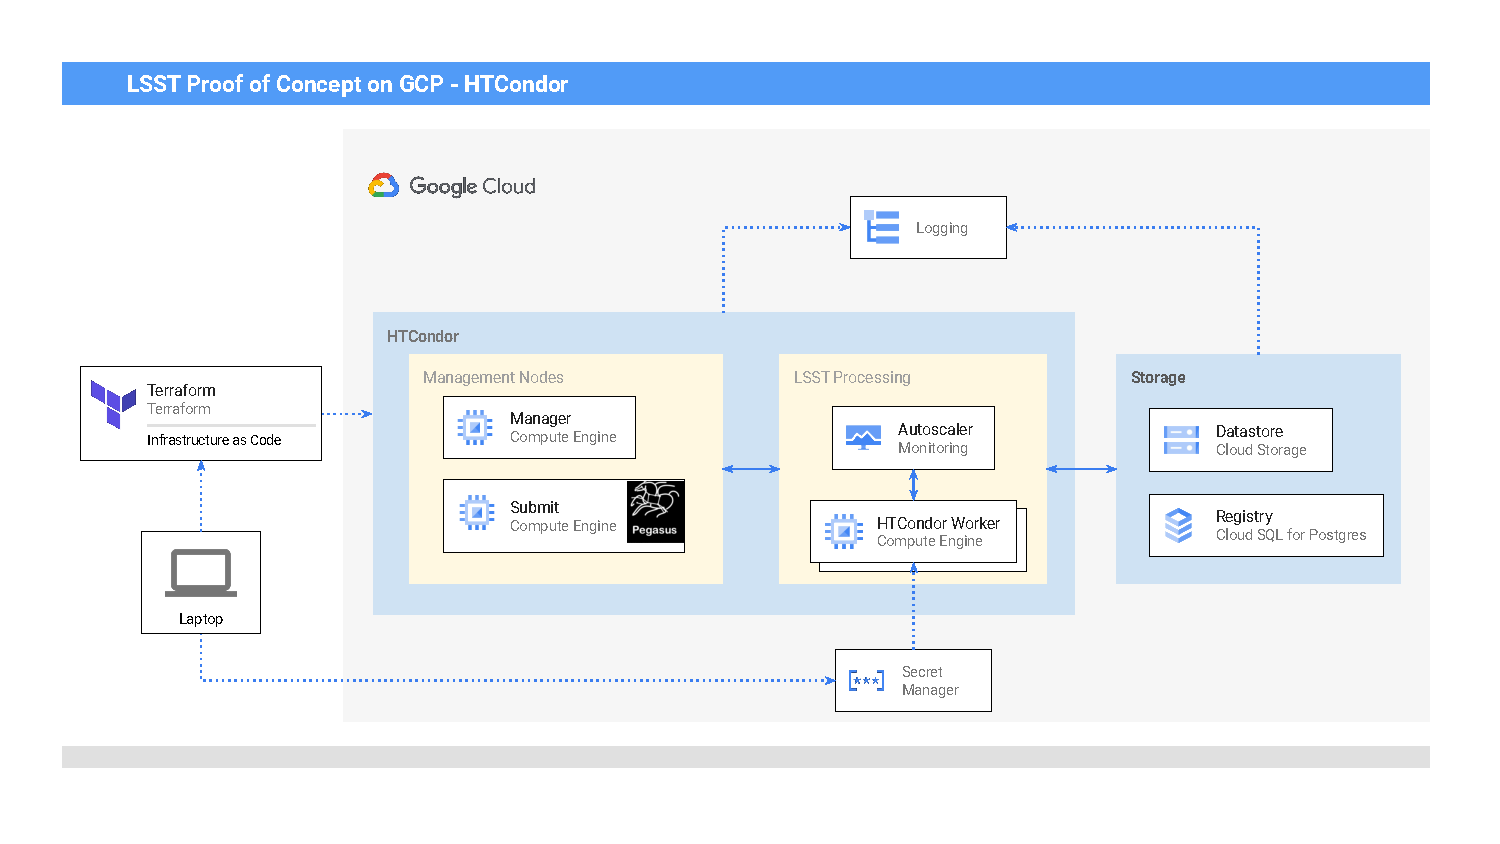
\includegraphics[width=1.0\textwidth]{HTCondor_Architecture.pdf}
\caption{Architecture diagram of the overall system}
\label{fig:architecture}
\end{figure}

The overall system architecture is shown in Figure \ref{fig:architecture}.
All components are hosted on Google Cloud Platform (GCP) except Terraform, which is infrastructure as code running from a laptop.
The LSST Science Pipelines Software Stack contains the applications for image processing and analysis.
A machine image based on a recent stack release together with other necessary software is built using Packer scripts.
The LSST Generation 3 Middleware, including Data Butler and PipelineTask framework, is used for this PoC.
The Butler datastore is a S3 compliant storage on Google Cloud Storage (GCS); objects are accessed using the \texttt{boto3} library.
The Butler registry is a Google Cloud SQL PostgreSQL database.
The usage of Data Butler is similar to the AWS PoC \citedsp{DMTN-137}, but the stack version is new.
Credentials to access the GCS bucket and the PostgreSQL instance are stored in Google Secret Manager; each machine retrieves the credentials and stores them in its local environments.


Google Compute Engine (GCE) deployed via Terraform provides the compute resources.
HTCondor is the underlying workload management system for batch jobs.
Pegasus is used on top of HTCondor for workflow submission and monitoring.
The HTCondor pool is automatically scaled with the load via a Managed Instance Group.
The HTCondor execute machines, or workers, can be either on-demand VMs or Preemptible VMs.
HTCondor Annex is an alternative to acquire cloud compute resources, but we did not use HTCondor Annex yet in this PoC due to time constraints (Sect \ref{sec:future}).
The stackdriver-based Cloud Monitoring and the fluentd-based Cloud Logging are turned on in the HTCondor cluster.
Pipeline logs are also sent to Cloud Logging, so we can search and examine logs in the Logs Viewer for troubleshooting.
(Note that the logging is not fully integrated yet, but is already useful.)


\subsection{Execution Results}

\subsubsection{Test runs}

Similar to \citeds{DMTN-137}, we first executed the \texttt{ci\_hsc} workflow, scaled up to process one tract HSC-RC2 dataset (\jira{DM-11345}), and then the full HSC-RC2 dataset.
So far, execution involved some manual intervention steps and has not been fully automated yet.
The overall steps were: Butler repo setup, QuantumGraph generation, workflow generation, and job execution.
To create a Butler repo on GCP after creating the GCS bucket and the PostgresSQL database, the bootstrap script at \url{https://github.com/lsst-dm/gen3-hsc-rc2} was run from the Verification Cluster located at NCSA to transfer the data to the GCS bucket and populate the Butler repo.
We did not optimize this step and it took around 40 hours for the full HSC-RC2 repo.
It can be improved by copying the data to the GCS first and creating the Butler repo from GCE.
We may also parallelize the ingestion process in the future.

In the Generation 3 Middleware, each executable unit is represented by a Quantum, and the DRP workflow is represented as a Quantum Graph with Quanta interdependency.
For the execution workflow, we added one initialization job and translated Quanta into jobs in the Pegasus format with one-to-one mapping.
For simplicity we considered all jobs of MakeWarpTask, CompareWarpAssembleCoaddTask, DeblendCoaddSourcesSingleTask, and MeasureMergedCoaddSourcesTask as large-memory jobs and required 30GB of memory.
Pegasus also added other necessary jobs to the execution workflow, such as data transfer of Quantum files and log files.
We used the submit node as the staging site, in the same manner as the AWS PoC \citedsp{DMTN-137}.

With the LSST software stack version \texttt{w\_2020\_30}, the tract \texttt{tract=9615} contains 26688 PipelineTask Quanta.
Table \ref{tab:taskBreakdownW30} shows an example run; this is comparable to Table 1 in \citeds{DMTN-137} and most differences were likely resulted from the LSST software stack version differences.
\begin{table}
\centering
\begin{tabular} {|r|r|r|}
\hline
{Task}&{Count}    &{Mean Runtime (sec)} \\ \hline
Init & 1 & 27.0 \\
IsrTask & 6765 & 58.6 \\
CharacterizeImageTask & 6765 & 169.9 \\
CalibrateTask & 6765 & 85.7 \\
MakeWarpTask & 4206 & 68.6 \\
CompareWarpAssembleCoaddTask & 405 & 424.9 \\
DetectCoaddSourcesTask & 405 & 88.6 \\
MergeDetectionsTask & 81 & 152.6 \\
DeblendCoaddSourcesSingleTask & 405 & 276.1 \\
MeasureMergedCoaddSourcesTask & 405 & 2541.4 \\
MergeMeasurementsTask & 81 & 40.0 \\
ForcedPhotCoaddTask & 405 & 3780.1 \\
\hline
%Total&26689   & \\ \hline
\multicolumn{2}{|r|}{Workflow wall time} & 8 hrs 52 mins \\
\hline
\multicolumn{2}{|r|}{Cumulative job wall time} & 61 days 5 hrs \\
\hline
\end{tabular}
\caption{Task breakdown of the HSC-RC2 tract=9615 workflow for the 20200729T200516 run.
There were 26688 pipeline jobs in total.
The mean runtime was the time spent on the resource as seen by Condor DAGMan.
The minimum runtime of the Pipetasks was 7.5 sec and the maximum was 6784.9 sec.
The software stack was \texttt{w\_2020\_30}.
}
\label{tab:taskBreakdownW30}
\end{table}

%\input{taskBreakdown_v20.tex}
%\input{runSummaryOneTract.tex}

The full HSC-RC2 dataset contains 3 tracts and around 1.5TB of input data, including 767 GB of raw images.
Currently we ignore narrow bands, so there are 404 visits in total.
One full HSC-RC2 workflow generates around 10TB of output data.
Using the stack version \texttt{w\_2020\_30}, the QuantumGraph generation took around 13 hours for the full HSC-RC2 dataset, resulted in 117388 Quanta in total in our test workflow.
We excluded patches that were not covered in all filters; this was a workaround as \texttt{CompareWarpAssembleCoaddTask} did not write out empty images which were expected in the QuantumGraph workflow.
The pipeline configurations can be found in \url{https://github.com/lsst-dm/google-poc-drp}.
When the workflow did not finish fully in one submission, we made a rescue workflow to run in another submission.
The rescue workflow only contained failed jobs or their dependents.
Making the rescue workflow required a manual step using a temporary patch in the \texttt{pipe\_base} package (\jira{DM-25809}), and took around 12 hours on one CPU.
Table \ref{tab:taskBreakdownFullW30} shows an example for the full HSC-RC2 workflow.

%\input{taskBreakdown_full_w30}
%\input{taskBreakdown_full_v20}
\begin{table}
\centering
\begin{tabular} {|r|r|r|r|r|}
\hline
{Task}&{Total Count}&{Count1}&{Count2}&{Mean Runtime (sec)} \\ \hline
Init    &    & 1 & 1 & 80.0 \\
IsrTask & 30278  & 30278 & 1 & 55.0 \\
CharacterizeImageTask & 30278& 30277 & 1& 129.2 \\
CalibrateTask & 30278 & 30277 & 1& 74.7 \\
MakeWarpTask & 20182 & 20180 & 2& 74.0 \\
CompareWarpAssembleCoaddTask & 1180 & 1178 & 2 & 700.3 \\
DetectCoaddSourcesTask & 1180 & 1178 & 2 & 105.2 \\
MergeDetectionsTask & 236 & 234 & 2 & 143.5 \\
DeblendCoaddSourcesSingleTask & 1180 & 1170 & 10 & 651.3 \\
MeasureMergedCoaddSourcesTask & 1180 & 1170 & 10 & 4426.7 \\
MergeMeasurementsTask & 236 & 234 & 2 & 40.7 \\
ForcedPhotCoaddTask & 1180 & 1170 & 10 & 6327.9 \\
\hline
\end{tabular}
\caption{
Example task breakdown of the HSC-RC2 workflow.
The mean runtime is the time spent on the resource as seen by Condor DAGMan in the 20200804T005441 + 20200806T041934 run using regular \texttt{n1-standard-8} machines.
Count 1 is the count from the first submission 20200804T005441; Count 2 is the count from the second, rescue submission 20200806T041934.
One IsrTask failed in the first submission and was retried in the second submission.
The software stack was \texttt{w\_2020\_30}.
}
\label{tab:taskBreakdownFullW30}
\end{table}


For the computes, we tested with GCP's first generation general-purpose machine types (N1) as well as the second generation general-purpose machine types (N2).
N2 provides better price-performanance and is used in the IDF quotes.
More specifically, the N1 machine \texttt{n1-standard-8} with 8 vCPUs and 30 GB of memory, and the N2 machine \texttt{n2-standard-8} with 8 vCPUs and 32 GB of memory were used.

The same HSC-RC2 workflow was run with multiple setups:

\begin{enumerate}
\item
Using on-demand N1 VMs as workers. Maximum 800 CPUs (100 VMs) simultaneously.
\item
Using on-demand N2 VMs as workers. Maximum 800 CPUs (100 VMs) simultaneously.
\item
Using preemptible N1 VMs as workers. Maximum 1600 CPUs (200 VMs) simultaneously.
\item
Using preemptible N2 VMs as workers. Maximum 1600 CPUs (200 VMs) simultaneously.
\end{enumerate}

Table \ref{tab:runSummary} summarizes the compute time of the runs.
Non-preemptible instances were used as HTCondor master and submit nodes.
\begin{table}
\tiny
\centering
\begin{tabular} {|c|c|c|c|c|c|}
\hline
Run & Setup & Max CPUs & Workflow walltime & Cumulative job time & Compute cost \\
\hline
20200731T011149+20200802T164424 & on-demand N1 workers     & 800  & 55 hrs & 308 days & \$1592 \\
20200804T005441+20200806T041934 & preemptible N1 workers & 1600 & 36 hrs & 275 days, 22 hrs & \$459  \\
20200806T215620+20200808T170615 & preemptible N2 workers & 1600 & 25 hrs & 213 days, 10 hrs & \$390  \\
20200811T172329                 & on-demand N2 workers     & 800  & 31 hrs & 300 days, 2 hrs  & \$1191 \\

20200814T002816+20200816T060623 & preemptible N2 workers & 1600 & 29 hrs & 208 days, 22 hrs & \$388 \\
\hline
\end{tabular}
\caption{
Run summary of the HSC-RC2 workflow with different setups.
The workflow wall time only includes Pegasus records, and may be dominated by random job failures and the rescue graph.
The costs are overestimates.
The Postgres instance size was increased between the 20200802T164424 run and the 20200804T005441 run; it stayed the same afterwards.
}
\label{tab:runSummary}
\end{table}



\subsubsection{Experienced Errors}
\begin{enumerate}
\item \textbf{GCS 403 HTTP error}.
Since we started large scale testing in early July, random 403 errors were received when Butler made HeadObject calls:
\begin{lstlisting}[style=basherror]
botocore.exceptions.ClientError: An error occurred (403) when calling the HeadObject operation: Forbidden
\end{lstlisting}
The stack interpreted it as
\begin{lstlisting}[style=basherror]
PermissionError: Forbidden HEAD operation error occurred. Verify s3:ListBucket and s3:GetObject permissions are granted for your IAM user.
\end{lstlisting}
However, the permission setup was the same for all jobs but only a very small fraction of jobs encountered this.
Butler did a HeadObject to check if an object existed before attempting to upload.
If the object did not exist it expected a 404 error.
At the time we used the \texttt{v20} stack and did not retry failed HTTP requests.
(A request-level retry using the \texttt{backoff} library was added by Dom Zippilli afterwards.)
A Google Cloud Support Ticket was filed to investigate the root cause, and concluded that there were transient issues at the IAM server during the same timeframe.
The instability of the IAM server was fixed on July 22.
We have not seen this error since.


\item  \textbf{Butler IntegrityError}
Conflicts of datasets were found occasionally when pipelines attempted to write outputs, for example:
\begin{lstlisting}[style=basherror]
  File "/opt/lsst/software/stack/conda/miniconda3-py37_4.8.2/envs/lsst-scipipe-1a1d771/lib/python3.7/site-packages/sqlalchemy/engine/default.py", line 590, in do_execute
    cursor.execute(statement, parameters)
psycopg2.errors.UniqueViolation: duplicate key value violates unique constraint "dataset_collection_24cc_unq_dataset_type_id_collection_c55de2f4"
DETAIL:  Key (dataset_type_id, collection_id, instrument, detector, visit)=(119, 60, HSC, 88, 1308) already exists.

  File "/opt/lsst/software/stack/conda/miniconda3-py37_4.8.2/envs/lsst-scipipe-1a1d771/lib/python3.7/site-packages/sqlalchemy/engine/default.py", line 590, in do_execute
    cursor.execute(statement, parameters)
sqlalchemy.exc.IntegrityError: (psycopg2.errors.UniqueViolation) duplicate key value violates unique constraint "dataset_collection_24cc_unq_dataset_type_id_collection_c55de2f4"
DETAIL:  Key (dataset_type_id, collection_id, instrument, detector, visit)=(119, 60, HSC, 88, 1308) already exists.


lsst.daf.butler.registry._exceptions.ConflictingDefinitionError: A database constraint failure was triggered by inserting one or more datasets of type DatasetType(src, {abstract_filter, instrument, detector, physical_filter, visit_system, visit}, SourceCatalog) into collection 'hfc18'. This probably means a dataset with the same data ID and dataset type already exists, but it may also mean a dimension row is missing.
\end{lstlisting}

In the scenario that a pipeline job was killed after partial outputs were written due to a machine shutdown, the follow-up process would redo the job and attempt to write all outputs.
Butler did not allow duplicate datasets nor overwriting existing datasets, hence a conflict error occurred.
This was expected and understood on preemptible machines; \jira{DM-26131} discusses how to handle preemption notice with a possible shutdown script and complete cleanup actions before the instance stops.
However, machine reboot can happen to regular machines too and we encountered the same error occasionally.
Closer investigation revealed that shutdown of regular instances due to maintenance events on the host machines can be mitigated with the live migrate option.
Since we started using the live migrate option we have not seen the issue.
Furthermore, \jira{DM-25818} removed the file existence check and allowed overwrite the stored file; the ticket was merged after the \texttt{w\_2020\_30} release.

% getting the above errors with different tasks and data.  The file should not have existed when the job started.  If I checked after I saw the error, the file can be found in the S3 datastore. Existing files have timestamp earlier than the failed job started.

\item  \textbf{Database size}
When we scaled up the number of workers without a sufficiently large Postgres instance, we encountered database operational errors such as:

\begin{lstlisting}[style=basherror]
sqlalchemy.exc.OperationalError: (psycopg2.OperationalError) FATAL:  remaining connection slots are reserved for non-replication superuser connections
\end{lstlisting}

and

\begin{lstlisting}[style=basherror]
Failed to build graph: (psycopg2.errors.ConfigurationLimitExceeded) temporary file size exceeds temp_file_limit (1025563kB)
\end{lstlisting}

As the number of simultaneous connections increased, it was expected that the Postgres instance needed to scale up.
These errors disappeared once the machine CPUs, memory, or the database flags such as \texttt{max\_connections} or \texttt{temp\_file\_limit} of the database instance were increased.

\item  \textbf{Other database issues}
There were more kinds of database operational errors, such as:

\begin{lstlisting}[style=basherror]
  File "/opt/lsst/software/stack/conda/miniconda3-py37_4.8.2/envs/lsst-scipipe-1a1d771/lib/python3.7/site-packages/sqlalchemy/engine/default.py", line 590, in do_execute
    cursor.execute(statement, parameters)
psycopg2.OperationalError: server closed the connection unexpectedly
        This probably means the server terminated abnormally
        before or while processing the request.
\end{lstlisting}

\begin{lstlisting}[style=basherror]
sqlalchemy.exc.OperationalError: (psycopg2.OperationalError) could not connect to server: No such file or directory
	Is the server running locally and accepting
	connections on Unix domain socket "/var/run/cloud-sql-proxy/light-team-275220:us-central1:drp-rc2-w30/.s.PGSQL.5432"?
\end{lstlisting}

These errors appeared to reduce with a larger database size per maximum simultaneous processes, but did not disappear completely.
The source of the error remains unclear.
In the current stack, Butler expects a long-lived database connection during pipeline execution and the connection pooling is disabled which might lead to unanticipated connection churns (\jira{DM-26302}).
We also see errors from the rate limit of the Cloud SQL Admin API calls.
When worker instances are added to the HTCondor cluster by the instance group autoscaling, there can be a surge of such Cloud SQL Admin API calls as the Cloud SQL Proxy starts in each instance.
It could be a quota limit or an issue in the code or configuration of the Google Cloud SQL Proxy, or something not yet considered.
We intend to investigate the source of the issue further.


\item  \textbf{Other rare transient errors}
For example, we occasionally saw
\begin{lstlisting}[style=basherror]
urllib3.exceptions.ProtocolError: ('Connection aborted.', OSError(0, 'Error'))
botocore.exceptions.ConnectionClosedError: Connection was closed before we received a valid response
\end{lstlisting}
It was very rare and working as expected.

\end{enumerate}


\subsection{Cost Analysis}
On GCP, the daily billing data can be exported to a BigQuery dataset and analysis can be done through SQL queries.

\subsubsection{GCS}
The GCS charge is dominated by the data storage cost, which is \$0.02 per GB per month for standard storage.
Storing 10 TB of the HSC-RC2 outputs costs \$200 per month.
As we operate completely within the GCP in the same region, there is no egress charge.
If we transferred 10 TB out of Google Cloud, it would cost around \$1110 in the normal rate; but there is a special offer to Internet2 Higher Education members and the National Research and Education Network (G\'{E}ANT NRENs) members, and data egress fees may be waived up to a maximum discount of 15\% of the total monthly Google Cloud fees.
Besides storage, for each run of HSC-RC2 workflow, the operations usage was typically less than \$4.

\subsubsection{Cloud SQL}
A PostgreSQL instance with 10 vCPUs, 65 GB of memory, and 15 GB of SSD storage was used and cost around \$23 per day while we ran the tests.
Storage capacity can be incrementally increased as needed.

\subsubsection{Compute}
Table \ref{tab:runSummary} summarizes the compute cost of running the HSC-RC2 workflow in different setups.
The workflow wall time was likely dominated by non-deterministic factors such as which jobs happened to fail and the size of the rescue workflow, therefore not very meaningful currently.
Instances were also underutilized during to the manual part of the workflow.
For example, the HTCondor cluster was left idle while the rescue workflow was made.
We have not optimized the overall usage.
Based on our limited tests, using N2 gave some performance boost with lower cost.
Each run using preemptible N2 workers cost about \$390.

\subsubsection{Cost projection}
We use the full run of the HSC-RC2 dataset with preemptible N2 workers to extrapolate the cost.
For each processing run through the DRP workflow, the total cost was roughly \$390 (GCP) + \$46 (Cloud SQL for 2 days) + \$17 (GCS) = \$453.
Note that it included all 3 tracts of the HSC-RC2 dataset, which was 4.5 times larger than the single-tract run used for cost analysis in \citeds{DMTN-137} with regard to the input raw CCD images.
With the dataset size in consideration, the run on GCP was roughly 6\% more expensive than the estimated cost in \citeds{DMTN-137}.
However, factors such as the database size, machine setups, manual intervention, and the rescue workflow can easily cause more than 10\% of differences in cost.
For example, in the AWS PoC we did not have a rescue workflow and only used the runs without failures.
Less clock time implied less cost from the database.
If we only considered 1 day of Cloud SQL usage, the cost would be about the same as the estimated cost on AWS.
In other words, the cost differences on GCP and on AWS were not significant in our test runs if we only look at list pricing.
Note that this report is not intended to cover commercial discounts and incentives which might change the pricing conclusion significantly.

\subsection{Future Improvement} \label{sec:future}

As the HSC-RC2 dataset is much smaller than the original target size, we will continue to scale up the data volume.

Other possible improvements include:
\begin{enumerate}
\item Use HTCondor Annex.
\item Use high-memory machine types.
\item Add native GCS Butler datastore rather than using its S3 interface.
\item Move the staging site. In this PoC we used the submit node as the staging site. \citet{Bektesevic2020} found that moving the staging to S3 can lead to better performance and reduce cost by 40-60 percent.
\item Improve failure recovery and eventually use retry features from the workflow manager. Newer version of the stack has some overwriting features.
\item Supply a shutdown script to handle the machine preemption (\jira{DM-26131}). This might mean a pipetask feature to clean up the unfinished work.
\item Improve efficiency of the scripts and automate the manual parts of the execution.
\item Fully integrate pipeline logs into Google Logging.



\end{enumerate}

\subsection{Summary}
Using a similar system architecture from the AWS PoC \citedsp{DMTN-137}, we were able to conduct DRP test runs with a recent DM stack on GCP.
The number of simultaneous jobs peaked at 1600, the largest we have tested in the cloud environments so far.
Based on our test runs, the estimated cost on GCP is about the same as the estimate on AWS.
